\chapter{TinyOS and NesC}

\section{The NesC language}

Recall traditional C code. In essence it consists of function
definitions and variable declarations listed in some order.  Calling
one function, causes a cascade of other calls, that eventually gets
useful work done. But how to know which function to call? Typically one
would find that out in documentation.

\subsection{Modules and interfaces}

In NesC\footnote{For a deeper discussion of the language see
\cite{NesC}}, above issue, is solved more systematically.  Each C code
file must {\bf provide} interfaces, and only through them it's
functions may be called. An {\bf interface} is nothing more but a set
of function names that are implemented in the file that provides it.
We call such, an interface enriched C file, a {\bf module}.

If interfaces can expose functions to external modules than, by
symmetry, there must also be a way to call functions exposed by those
external modules. To accomplish that, NesC module is not only allowed
to provide interfaces, but can also {\bf use} them. If a module declares to
use an interface, than it's free to call any function this interface
contains. At this point, it isn't however decided where interfaces, it
declares to use, will be implemented. It merely states that it will
need them.

Summarizing, a module is a C file that provides a set of interfaces
and uses a different set of interfaces to help it do the work. This
decomposition of an application, that used to be global, into module
sized pieces makes complexity much easier to manage. Moreover,
dependencies between modules are now explicitly stated. To understand
inner workings of a module you only need to see it's code and the code
of interfaces it declares to use or provide.

\subsection{Configurations}

We didn't yet mention, how a module that uses an interface, gets
paired with one that provides it. This is done, through a new type of
a file, called a {\bf configuration}. Configurations however, do much
more than just connecting interfaces of modules together.

Firstly they can use and provide interfaces just as modules
do\footnote{Though only modules contain actual function
implementations.}. In fact modules and configurations are so similar
than we jointly name them {\bf components}.

Secondly they can instantiate components. By default all components
(modules and configurations) are singletons. If a singleton component
isn't ever instantiated in an application, it isn't considered during
compilation.

Each configuration first instantiates all components it intends to
work with. Then it defines connections between their interfaces. And
finally, if it has declared to use or provide any interfaces, it passes
these interfaces to components it instantiated.  This means that an
interface provided by a configuration, may be passed through several
layers of configurations until it finally is implemented by some
module.

This mechanism forms basis for creating {\bf self-contained hermetic
abstractions}. Namely, a top level configuration can provide a set of
useful interfaces and hide all their implementation details. Said
implementation can utilize several layers of abstraction, connect
itself to components shard within application and manage module
initialization, but user doesn't have to know any of it. All he will
have to do, is instantiate this top level configuration in his
application and make use of provided interfaces\footnote{In fact, each
TinyOS application is such a high level configuration, that pulls in
all dependencies and connects them to the module that implements
application logic.}.

We will use graphical representation of components, suggested in
\cite{UML2ForTOS} (see Figure \ref{fig:example_component}) and where
it's relevant, we'll distinct modules from configurations by adding
\emph{<<realization>>} or \emph{<<specification>>} stereotypes
respectively.

\begin{figure}[h]
  \centering
  \includegraphics{diagrams/example_component.eps}
  \caption{Component with one provided and one used interface.}
  \label{fig:example_component}
\end{figure}

\subsection{Two-way interfaces}

NesC interfaces are in fact {\bf two-way}. To explain this concept,
we'll consider an example, where user requests an asynchronous
operation. One possible way to support this through interface
connections is shown in Figure \ref{fig:two_way_interface1}. The user
calls \emph{start()} to initiate the operation and provider calls
\emph{completed()} to notify user about it's completion.

\begin{figure}[h]
  \centering
  \includegraphics{diagrams/two_way_interface1.eps}
  \caption{Asynchronous operation implemented with two interfaces.}
  \label{fig:two_way_interface1}
\end{figure}

Though this scheme works, it forces the use of two connections where
there is only one logical association. Need to connect callbacks
separately from requests is an unnecessary nuisance. Instead NesC allows
{\bf events} to be part of interfaces, in addition to normal function
calls known as {\bf commands}. User of such interface will have to
implement handlers for all events, which again are nothing more than C
functions with proper names. Above scheme, implemented using events,
is shown in Figure \ref{fig:two_way_interface2}.

\begin{figure}[h]
  \centering
  \includegraphics{diagrams/two_way_interface2.eps}
  \caption{Asynchronous operation implemented with a two-way interface.}
  \label{fig:two_way_interface2}
\end{figure}

\subsection{Parametrized interfaces}
A component may provide a vitalized resource. This means that a real
resource is split by software to serve several users. For example,
let's consider the problem of waking a group people in a hotel.
Everyone wants to be woken at different hours, but manager only has a
single alarm clock. Solution is simple, he has to set the alarm for
himself, to the nearest waking time of one of his customers. Then, when it
fires, he can wake that person up and reset the alarm to the next
nearest waking time. In essence this scheme crates multiple alarm
clocks using only one. We may say that it virtualizes the alarm clock
\footnote{This is actually a practical problem in low level
programming. Few hardware timers need to be virtualized, to serve
multiple software components.}.

In NesC this would correspond to providing several \emph{Alarm}
interfaces, while using only one. Exactly how many of these virtual
interfaces should be provided, isn't however known ahead of time.
Moreover, if for each virtualized interface, separate function
implementations were needed, it would lead to wasteful code
duplication.

Instead NesC offers {\bf parametrized interfaces}. They differer from
regular interfaces in that each implementing function receives an
additional parameter denoting number of the interface that was used to
call it. Notice that this is by far the most convenient way to
implement our alarm replicator, because it can use this additional
argument to index and update an array of firing times and then easily
find the closest one. Exemplary replication of the \emph{Alarm}
resource is presented in Figure~\ref{fig:parametrized_interface}

\begin{figure}[h]
  \centering
  \includegraphics[width=0.9\textwidth]{diagrams/parametrized_interface.eps}
  \caption{Parametrized interface used in timer virtualization.}
  \label{fig:parametrized_interface}
\end{figure}

\subsection{Generic components}

Implementing a data structure like \emph{BitVector} as a singleton,
doesn't make much sens. Therefore NesC allows for a component to be
made {\bf generic}. Making a module or configuration generic has two
major consequences.  Firstly all it's instantiations will create
separate and independent components, just as if the code was copied.
Secondly it is possible to pass arguments (both type and value) that
will parametrize such newly created component. Graphically, generic
components are distinguished by the parentheses after their name, as
in Figure~\ref{fig:generic_component}. Also note that interfaces can
be type parametrized as well, because it well supplements generic
components.

\begin{figure}[h]
  \centering
  \includegraphics{diagrams/generic_component.eps}
  \caption{A generic component with type and integer arguments,
  providing a parametrized interface.}
  \label{fig:generic_component}
\end{figure}

\subsection{Memory allocation}
Many errors found on wireless sensor nodes, for which software was
written in C, were caused by various memory related errors. Failed
allocation due to lack of available memory and leaks were problems
particularly painful on nodes with very limited resources.

For this reason, in NesC all memory allocation is static and resolved
during compilation. This way, compiler can easily detect if the
required amount of memory exceeds the amount available on the device.

\section{The TinyOS operating system}

\begin{quotation}
TinyOS is an open source, BSD-licensed operating system designed for
low-power wireless devices, such as those used in sensor networks,
ubiquitous computing, personal area networks, smart buildings, and
smart meters. A worldwide community from academia and industry use,
develop, and support the operating system as well as its associated
tools, averaging 35,000 downloads a year.

It started as a collaboration between the University of
California, Berkeley in co-operation with Intel Research and Crossbow
Technology, and has since grown to be an international consortium, the
TinyOS Alliance.

{\hfill \cite{TOSnet,TOSw}}
\end{quotation}
TinyOS is written in NesC programming language. This means, that its
made of components which interact with each other only through,
separately specified, interfaces. The great advantage of this is
that these components have very clear boundaries and its easy to
understand how to use them. Consider example\footnote{This isn't a
cleverly chosen example. Components tend to be this intuitive.} shown
in Figure~\ref{fig:platform_serial}.
\begin{figure}[h]
  \centering
  \includegraphics{diagrams/platform_serial.eps}
  \caption{\emph{PlatformSerialC} gives access to the serial port of the 
           Chronos watch.}
  \label{fig:platform_serial}
\end{figure}
Its obvious, that first you need to call \emph{start()}, then send
bytes with \emph{send()} method and optionally call \emph{stop()} when
serial port is no longer needed. Complex details of handling the
hardware are hidden beneath the abstraction.

Another TinyOS's advantage is its portability. Officially it comes
with support for 22 platforms and many more are available through
various project forks. It also comes with many applications that share
its core components, and most of them are platform independent. This
results in a cartesian cross of platforms and applications, which is
incomparably more effective, that having application and platform
tied together.

Testing is also well supported on TinyOS. Firstly, a whole-network
simulator \cite{TOSSIM} is available. It alows to simulate the
software of not one, but a whole network of nodes, on a PC. Moreover
its radio connectivity models are precise enough to draw, resonably
realistic, conclusions from the simulations. {\bf TOSSIM} is an
envaluable tool for TinyOS developers. Secondly, a NesC unit-testing
framework \cite{TOSMock}, has been recently added to TinyOS. {\bf TOSMock}'s
ability to verify each component's behaviour gratly supplements
high level testing provided by TOSSIM.






% Vim settings:
% vim: set textwidth=70:
% vim: set fo+=t:
